\documentclass[11pt]{article}
\pdfinfoomitdate=1\pdftrailerid{}
\usepackage[letterpaper,margin=.7in,headheight=15pt,headsep=18pt,footskip=24pt]{geometry}
\usepackage[T1]{fontenc}\usepackage{lmodern,amsmath,amssymb,array,booktabs,fancyhdr,tikz}
\usetikzlibrary{arrows.meta}\usepackage{sansmath}\usepackage{needspace}
\renewcommand{\familydefault}{\sfdefault}\setlength{\parindent}{0pt}\setlength{\parskip}{6pt}
\pagestyle{fancy}\fancyhf{}\fancyhead[L]{\small Week NN / Pancake flips / Facilitator guide}
\fancyfoot[L]{\scriptsize Bellingham Math Circle / Week NN / NN-FAC-v1}\fancyfoot[R]{\thepage}
\newcommand{\head}[1]{\par\textbf{\large #1}\par}
\newcommand{\sub}[1]{\par\textbf{#1}\par}
% a pancake whose dark side faces up
\newcommand{\up}[1]{$\overline{#1}$}
\definecolor{cakefillc}{RGB}{248,224,170}\definecolor{cakedrawc}{RGB}{140,95,35}
\tikzset{cakefill/.style={fill=cakefillc}, cakedraw/.style={draw=cakedrawc, line width=0.7pt},
  platedraw/.style={draw=black!55, line width=0.5pt}, platefill/.style={fill=black!18}}
\begin{document}\sansmath
\head{Mathematical overview: a method sets an upper bound, breaks set a lower bound}
\textbf{The model.} Pancakes $1,\dots,n$ (1 smallest) form a stack, written as its numbers from the top. It is sorted when it reads $1\,2\,\dots\,n$, each pancake on a bigger one. \emph{Flip $k$} slides the spatula under the $k$-th pancake from the top and turns the top $k$ over as one block, which reverses their order. Flip 1 changes nothing for plain pancakes. ``A stack needs $k$ flips'' always means the fewest flips that sort it.

\textbf{Every flip undoes itself.} Doing flip $k$ twice restores the stack. So the flips that sort a stack, done in reverse order, build it from $1\,2\,\dots\,n$: a stack is as many flips from sorted as sorted is from it. Working outward from the sorted stack (one flip away, then two, and so on) lists every stack by the flips it needs; this makes each ``find all'' answer complete. For four pancakes the layers hold 1, 3, 6, 11 and 3 stacks (table, guide page~\pageref{tab:four}).

\textbf{Upper bound: two flips per pancake, at most $2n-3$ flips ($n\ge2$).} Flip the biggest pancake not yet in place to the top, then flip it down into its place. A placed pancake lies below every later spatula and never moves again, so each pancake costs at most two flips, and the last two pancakes need at most one flip between them: $2(n-2)+1=2n-3$. That is 9 for six, 17 for ten and 37 for twenty. This method really uses $2n-3$ on some stacks (9 on $2\,6\,5\,1\,3\,4$; checked for $n\le7$), but it is not the fastest: it takes 8 flips on $3\,6\,1\,5\,2\,4$, which needs 6.

\textbf{Lower bound: breaks.} Stand the stack on a plate numbered $n+1$. A \emph{break} is a touching pair, two pancakes or the bottom pancake and the plate, whose numbers differ by more than 1. Only a sorted stack has no breaks: reading up from the plate, each number must be one less than the one below. A flip keeps every touching pair inside the lifted block (reversed) and below it; the only new pair is at the spatula, where the old top pancake meets the pancake, or the plate, below the block. So one flip removes at most one break, and \emph{a stack with $b$ breaks needs at least $b$ flips}. The bound is often not reached: $1\,3\,2$ has 2 breaks and needs 3; $2\,1\,4\,3\,6\,5$ has 3 and needs 5; $4\,6\,2\,5\,1\,3$ has 6 and needs 7. Sharper: a $b$-flip sort must remove a break with every flip, so following only break-removing flips either sorts the stack in $b$ or proves $b$ is not enough.

\textbf{The worst stacks.} The most flips any stack needs are 1, 3, 4, 5, 7, 8 for 2 to 7 pancakes (computer, every stack). The worst stacks are $1\,3\,2$ for three; $4\,2\,3\,1$, $2\,4\,1\,3$ and $3\,1\,4\,2$ for four; 20 stacks for five; $4\,6\,2\,5\,1\,3$ and $5\,3\,6\,1\,4\,2$ for six. For large stacks the exact worst case is unknown; Gates and Papadimitriou proved that $(5n+5)/3$ flips always suffice, and exact values are known only up to 19 pancakes (from the sources, not checked here).

\textbf{Dark sides (burnt pancakes).} Each pancake has a dark side that must end facing down. A flip also turns each lifted pancake over, so flip 1 now matters, and flips still undo themselves. Bring the biggest pancake not in place to the top, turn it over alone if its dark side faces down, and flip it down, dark side down: at most three flips per pancake and one for the last, $3n-2$ (16 for six). The true maxima are 1, 4, 6, 8, 10, 12 for 1 to 6 pancakes (computer). With two pancakes only \up1\,\up2 needs 4 (a bar marks a dark side up); with three, exactly \up1\,\up2\,\up3 and $1$\,\up2\,\up3 need 6.

\textbf{Experiments, conjectures and explanations.} Sorting a stack in $k$ flips is an experiment that proves $k$ is enough for that stack. Failing to do better is evidence for a conjecture, not a proof. ``Needs at least $k$'' is proved by counting breaks, by checking every first move (a tree), or by the outward layers. The method's count and the break argument are the explanations of the two bounds. That no stack of five needs six, that seven flips therefore always suffice for six, and the worst counts beyond six are computer facts children can only conjecture; that $4\,6\,2\,5\,1\,3$ needs seven, 4--5 children can prove (Problem 6).

\textbf{Bands and prerequisites.} Children should discover that the biggest pancake can always be flipped into place, so every stack can be sorted; that some small stacks need surprisingly many flips; and (grades 4--5) that counting breaks proves a stack cannot be sorted faster. \emph{K--1} (no reading, as the adult reads; counting to about 10; writing or dictating digits) sorts stacks of three and four, finds all six stacks of three and every stack of four one flip sorts, and meets dark sides on two pancakes. \emph{Grades 2--3} (reading short problems; adding and doubling to about 20) sorts stacks of up to six, explains why $1\,3\,2$ needs three, counts a method that always works, finds all stacks of four that need four, and sorts dark-sided stacks. \emph{Grades 4--5} (spotting numbers that differ by more than 1; $2\cdot20-3$; following an argument about every possible flip) also proves both bounds, certifies the worst stacks of four and a worst stack of five, shows $4\,6\,2\,5\,1\,3$ needs seven, and extends the method to dark sides.
\newpage
\head{Preparation, shared launch and pacing}
\textbf{Status.} Prepared for organizer review; unpiloted. The materials sheet's sizes are measured in its PDF, but no set has been cut or handled. Not physically rehearsed: cutting the sets and whether the heavy brown ink makes card curl, the foam backing below, a card spatula slipping under one pancake, flipping a block of four to six as one unit, seeing a stack's order, and telling which side is dark inside a stack. Times are estimates.

\textbf{What to print.} The packets, one per child, single-sided US Letter at 100\%: K--1 4 pages, Grades 2--3 6 pages, Grades 4--5 7 pages. Nothing in them is cut and no page is a mat: the drawn pancakes are smaller than the real ones, so children build each stack beside its picture and rebuild from the picture when a stack gets lost. Materials page 1, ``Pancakes and spatula'': one copy per pair and one for the launch (six for the current group), single-sided on card stock at 100\%; its 100\,mm bar should measure 100\,mm.

\textbf{Making the sets.} Each copy of materials page 1 is one set: pancakes 1 to 6, 4 to 9\,cm across, and a spatula. The printed face, solid brown with a white number, is the dark side; the plain back is the light side. Cut out the six pancakes and the spatula, then write each number large on the back with a marker, underlining the 6. K--1 sets need only pancakes 1--4; the launch set can go to the 4--5 referee afterwards. Better if you can get it (untested): cut off the spatula, stick the rest of the sheet onto light-coloured 2\,mm self-adhesive craft foam, and cut the pancakes through both layers. Six card pancakes stand about 2\,mm tall, too thin to see their order from the side, so children must lift pancakes to check; a foam stack stands about 14\,mm and shows its layers. Keep the spatula plain card so it slips under one pancake. Preparation: about 30 minutes beyond printing with card alone (cutting 25, numbering the backs 5); allow 15 more for foam.

\textbf{Also needed.} Twelve counters per K--1 pair as flip tokens; pencils, as the older bands write their flips; a sticky-note pad for the 2--3 table (Problem 5) and the 4--5 table (Problem 4); optionally a paper plate to make the 4--5 plate concrete.

\textbf{Staffing.} With the current group, one adult stays at each table. The K--1 adult reads each problem aloud and watches, with the partner, that every flip turns the whole block over; the adult never chooses where the spatula goes and does not announce the fewest flips before a child has a count (``Can you do it in fewer?'' is the follow-up). The 2--3 adult asks each child for their method's count in Problem 4 and helps the table keep the sticky-note columns in Problem 5. The 4--5 adult listens to Problems 3, 4 and 6 and records the Problem 6 tree; the third child referees the whole-block rule and the counts, rotating. With only two adults, 2--3 and 4--5 can share one. Writing down flips a child calls out is ordinary support; an adult choosing flips means the stack is too big.

\textbf{Launch (whole group, about five minutes).} Hand out the sets and give a minute to handle them; ask for a tower with each pancake on a bigger one: ``That is a sorted stack. From now on the only move is a flip.'' Say that the brown sides do not matter until a page says so. On the launch set build $4\,3\,1\,2\,5$ from the top and show the rule: the spatula goes under any pancake, and everything above it turns over together. Not allowed: pulling a pancake out of the middle, flipping only the bottom part, or moving a block without turning it over. Do two flips, putting down a token for each:
\begin{center}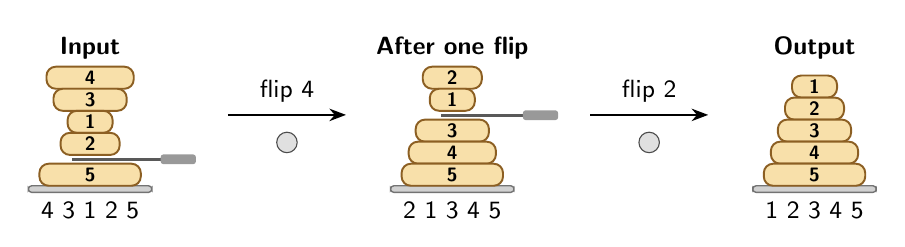
\begin{tikzpicture}
\draw[platedraw, platefill, rounded corners=0.042cm] (-0.784,-0.084) rectangle (0.784,0);
\draw[cakefill, cakedraw, rounded corners=0.118cm] (-0.554,1.232) rectangle (0.554,1.512);
\node[font=\scriptsize\bfseries, inner sep=0pt] at (0.000,1.372) {4};
\draw[cakefill, cakedraw, rounded corners=0.118cm] (-0.465,0.952) rectangle (0.465,1.232);
\node[font=\scriptsize\bfseries, inner sep=0pt] at (0.000,1.092) {3};
\draw[cakefill, cakedraw, rounded corners=0.118cm] (-0.286,0.672) rectangle (0.286,0.952);
\node[font=\scriptsize\bfseries, inner sep=0pt] at (0.000,0.812) {1};
\draw[cakefill, cakedraw, rounded corners=0.118cm] (-0.375,0.392) rectangle (0.375,0.672);
\node[font=\scriptsize\bfseries, inner sep=0pt] at (0.000,0.532) {2};
\draw[cakefill, cakedraw, rounded corners=0.118cm] (-0.644,0.000) rectangle (0.644,0.280);
\node[font=\scriptsize\bfseries, inner sep=0pt] at (0.000,0.140) {5};
\fill[black!65] (-0.235,0.316) rectangle (0.896,0.356);
\fill[black!40, rounded corners=1pt] (0.896,0.274) rectangle (1.344,0.398);
\node[anchor=north, font=\small, inner sep=0pt] at (0.000,-0.204) {4 3 1 2 5};
\node[font=\small\bfseries] at (0.000,1.750) {Input};
\draw[-{Stealth[length=6pt]}, thick] (1.750,0.9) -- (3.250,0.9);
\node[above, font=\small] at (2.500,0.9400000000000001) {flip 4};
\draw[black!70, fill=black!12] (2.500,0.550) circle (0.13);
\draw[platedraw, platefill, rounded corners=0.042cm] (3.816,-0.084) rectangle (5.384,0);
\draw[cakefill, cakedraw, rounded corners=0.118cm] (4.225,1.232) rectangle (4.975,1.512);
\node[font=\scriptsize\bfseries, inner sep=0pt] at (4.600,1.372) {2};
\draw[cakefill, cakedraw, rounded corners=0.118cm] (4.314,0.952) rectangle (4.886,1.232);
\node[font=\scriptsize\bfseries, inner sep=0pt] at (4.600,1.092) {1};
\draw[cakefill, cakedraw, rounded corners=0.118cm] (4.135,0.560) rectangle (5.065,0.840);
\node[font=\scriptsize\bfseries, inner sep=0pt] at (4.600,0.700) {3};
\draw[cakefill, cakedraw, rounded corners=0.118cm] (4.046,0.280) rectangle (5.154,0.560);
\node[font=\scriptsize\bfseries, inner sep=0pt] at (4.600,0.420) {4};
\draw[cakefill, cakedraw, rounded corners=0.118cm] (3.956,0.000) rectangle (5.244,0.280);
\node[font=\scriptsize\bfseries, inner sep=0pt] at (4.600,0.140) {5};
\fill[black!65] (4.454,0.876) rectangle (5.496,0.916);
\fill[black!40, rounded corners=1pt] (5.496,0.834) rectangle (5.944,0.958);
\node[anchor=north, font=\small, inner sep=0pt] at (4.600,-0.204) {2 1 3 4 5};
\node[font=\small\bfseries] at (4.600,1.750) {After one flip};
\draw[-{Stealth[length=6pt]}, thick] (6.350,0.9) -- (7.850,0.9);
\node[above, font=\small] at (7.100,0.9400000000000001) {flip 2};
\draw[black!70, fill=black!12] (7.100,0.550) circle (0.13);
\draw[platedraw, platefill, rounded corners=0.042cm] (8.416,-0.084) rectangle (9.984,0);
\draw[cakefill, cakedraw, rounded corners=0.118cm] (8.914,1.120) rectangle (9.486,1.400);
\node[font=\scriptsize\bfseries, inner sep=0pt] at (9.200,1.260) {1};
\draw[cakefill, cakedraw, rounded corners=0.118cm] (8.825,0.840) rectangle (9.575,1.120);
\node[font=\scriptsize\bfseries, inner sep=0pt] at (9.200,0.980) {2};
\draw[cakefill, cakedraw, rounded corners=0.118cm] (8.735,0.560) rectangle (9.665,0.840);
\node[font=\scriptsize\bfseries, inner sep=0pt] at (9.200,0.700) {3};
\draw[cakefill, cakedraw, rounded corners=0.118cm] (8.646,0.280) rectangle (9.754,0.560);
\node[font=\scriptsize\bfseries, inner sep=0pt] at (9.200,0.420) {4};
\draw[cakefill, cakedraw, rounded corners=0.118cm] (8.556,0.000) rectangle (9.844,0.280);
\node[font=\scriptsize\bfseries, inner sep=0pt] at (9.200,0.140) {5};
\node[anchor=north, font=\small, inner sep=0pt] at (9.200,-0.204) {1 2 3 4 5};
\node[font=\small\bfseries] at (9.200,1.750) {Output};
\end{tikzpicture}
\end{center}
For the older tables write \emph{$4\,3\,1\,2\,5$, flips: 4 2}: a stack is its numbers from the top, a flip the number of pancakes it turns over. End with ``Your pages give you stacks to sort with as few flips as you can.'' Flip without saying why you chose those flips. This run, like the printed example ($3\,1\,2$ in two flips), flips the biggest pancake on top down into its place, which is half of the method that 2--3 Problem 4 and 4--5 Problem 2 ask for; do not name that pattern. Do not sort a printed stack or repeat a flip (that a flip undoes itself is for children to find).

\textbf{Dark sides, launched at the table.} Watch whether K--1 children assume the brown sides matter before a page says so. At a table's first dark-side problem (K--1 Problem 5, 2--3 Problem 6, 4--5 Problem 7), build the printed example, $2$\,\up1\,$3$, with the 1 brown side up, and do flip 2: the two pancakes swap and both turn over, giving $1$\,\up2\,$3$, in order but not finished. Say that the spatula under the top pancake turns just that one over. To record, shade a slot's top edge for a dark side up and its bottom edge for down, as in the pictures. Only the top face shows in a stack, so lift to check.

\textbf{A first visit.} After the opening and launch, allow 35--40 minutes of work and a few minutes to share one hardest stack and one method count. First route: K--1 Problems 1--3 (Problem 4 for a quick pair); Grades 2--3 Problems 1--4; Grades 4--5 Problems 1--4, but Problem 2 alone can take 15 minutes, so if time is short go from Problem 1 to Problems 3 and 4 and open the return visit with Problem 2. Return visit: K--1 Problems 4--6; Grades 2--3 Problem 5 (pooled), then 6--8; Grades 4--5 Problems 5 and 6, then 7--9. A 2--3 child who finishes can meet breaks in 4--5 Problem 3; a confident K--1 sorter can try 2--3 Problem 2 aloud. Finishing every page is not the goal.

\sub{All 24 stacks of four, by fewest flips (every band)}\label{tab:four}
The layers named in the overview, for checking K--1 Problems 2--4, 2--3 Problem 5 and 4--5 Problem 4.
\begin{center}\renewcommand{\arraystretch}{1.2}
\begin{tabular}{c l}
Fewest flips & Stacks of four (all 24, worked outward from $1\,2\,3\,4$)\\\midrule
0 & $1\,2\,3\,4$\\
1 & $2\,1\,3\,4$,\ $3\,2\,1\,4$,\ $4\,3\,2\,1$\\
2 & $2\,3\,1\,4$,\ $2\,3\,4\,1$,\ $3\,1\,2\,4$,\ $3\,4\,2\,1$,\ $4\,1\,2\,3$,\ $4\,3\,1\,2$\\
3 & $1\,2\,4\,3$,\ $1\,3\,2\,4$,\ $1\,3\,4\,2$,\ $1\,4\,2\,3$,\ $1\,4\,3\,2$,\ $2\,1\,4\,3$,\ $2\,4\,3\,1$,\ $3\,2\,4\,1$,\ $3\,4\,1\,2$,\ $4\,1\,3\,2$,\ $4\,2\,1\,3$\\
4 & $2\,4\,1\,3$,\ $3\,1\,4\,2$,\ $4\,2\,3\,1$
\end{tabular}\end{center}

\newpage
\head{K--1: sorting with tokens}
Each pair uses pancakes 1--4 and the spatula cut from materials page 1; Problems 5--6 use pancakes 1 and 2, brown face as the dark side. Before Problem 1, show the recording once with the printed example $3\,1\,2$, on scrap paper: the top slot is the top pancake, and when the stack is sorted, count the tokens into the flips box and clear them. The adult or partner may write numbers a child says.

Stacks are written from the top; ``flips 3 2'' means flip 3, then flip 2. A bar marks a pancake whose dark side faces up. In the pictures a dark band on a pancake's top edge means its dark side is up. Every count below is the fewest; children's own counts will often be higher, and that is fine.

\sub{Problem 1, page 1: all six stacks of three}
$1\,2\,3$ needs 0; $2\,1\,3$ needs 1 (flip 2); $3\,2\,1$ needs 1 (flip 3); $3\,1\,2$ needs 2 (flips 3 2, the printed example); $2\,3\,1$ needs 2 (flips 2 3); $1\,3\,2$ needs 3 (flips 2 3 2 or 3 2 3). Circle $1\,3\,2$. There are two stacks with each pancake on top, so six in all; the sorted stack counts as one of the six. A child's reason for $1\,3\,2$: ``I tried both first flips, and after either one it still took two more.'' The ``most flips'' depends on fewest counts, so if a box shows more than the number above, ask ``Can you do it with fewer tokens?'' before the circling. Hints: ``How will you know when you have all six?'' ``Is a sorted stack one of the ways?'' Extension: make a stack for your partner that needs exactly two flips.

\sub{Problem 2, page 2: four stacks of four}
$4\,1\,2\,3$: 2 (flips 4 3). $2\,3\,4\,1$: 2 (3 4). $3\,4\,2\,1$: 2 (2 4). $1\,2\,4\,3$: 3, and the only three-flip sort is 4 2 4, which begins by turning the whole stack over. Children often want to swap the 4 and 3 at the bottom, which no flip can do alone. Hint: ``Where must the 4 end up, and how can a flip get it there?''

\sub{Problem 3, page 2: every stack one flip sorts}
$2\,1\,3\,4$, $3\,2\,1\,4$ and $4\,3\,2\,1$, one for each blank. They are complete because the same flip undoes a sorting flip: these are exactly what one flip does to a sorted stack, with the spatula under pancake 2, 3 or 4 (under the top pancake nothing changes). ``Mixed-up'' leaves out $1\,2\,3\,4$. Hint: ``What do you get when you flip a sorted stack once? What if you do the same flip again?'' Extension: find stacks that need exactly two flips (six; table, guide page~\pageref{tab:four}).

\sub{Problem 4, page 3: three hard stacks and a decoy}
$4\,2\,3\,1$: 4 (flips 4 2 3 2). $2\,1\,4\,3$: 3 (3 4 3). $2\,4\,1\,3$: 4 (2 4 3 2). $3\,1\,4\,2$: 4 (2 3 4 2). The three four-flip stacks are the hardest stacks of four; $2\,1\,4\,3$ looks similar and needs only three. Expect first counts of 5 to 8. If a child says a stack ``can't be done in three,'' ask ``How could we be sure?'' and leave it open; the adult can say that grown-ups checked every way. To share: ``Which stack was hardest?''

\sub{Problem 5, page 4: dark sides on two pancakes}
\up1\,2: 1 (flip 1). \up2\,\up1: 1 (flip 2). \up2\,1: 2 (flips 2 1). $2\,1$, both dark down: 3 (1 2 1). The usual slip is flipping a block without turning each pancake over. Hint: ``After that flip, which way is each dark side facing?''

\sub{Problem 6, page 4: the hardest stack of two}
\up1\,\up2, 1 on 2 with both dark sides up, needs 4 (flips 1 2 1 2 or 2 1 2 1); it is the only one. All eight stacks: $1\,2$ needs 0; \up1\,2 and \up2\,\up1 need 1; \up2\,1 and $2$\,\up1 need 2; $2\,1$ and $1$\,\up2 need 3. With only eight stacks (two orders, four ways for the dark sides), the table can build them all. The three blank stacks are working space for candidates, not three answers. Hint: ``How many different stacks of 1 and 2 can you make?''
\newpage
\head{Grades 2--3: fewest flips, a method that always works}
Each pair uses a full set from materials page 1; Problems 6--8 use the brown face as the dark side.
\sub{Problem 1, page 1}
$2\,3\,4\,1$: 2 (flips 3 4). $3\,4\,1\,2$: 3 (2 4 2). $5\,4\,3\,2\,1$: 1 (5). $5\,1\,2\,3\,4$: 2 (5 4). $4\,5\,1\,2\,3$: 3 (2 5 3). $1\,2\,3\,5\,4$: 3 (5 2 5). Each shortest sort is the only one of its length. Hint: ``Where must the biggest pancake end up?''

\sub{Problem 2, page 2: the stack of three that needs the most}
$1\,3\,2$ needs 3 (flips 2 3 2). Why not two: flip 1 does nothing, so the first flip is flip 2, giving $3\,1\,2$, or flip 3, giving $2\,3\,1$. The only stacks one flip from sorted are $2\,1\,3$ and $3\,2\,1$, the sorted stack flipped once, and neither first flip lands on one. With the six stacks laid out, a child can show this by pointing. Breaks (4--5 Problem 3) give only 2 here. Hint: ``What could your first flip be? After it, could one more flip finish?''

\sub{Problem 3, page 2: stacks of six}
$6\,5\,4\,3\,2\,1$: 1 (flip 6). $3\,6\,1\,5\,2\,4$: 6, and only by 5 4 6 3 4 5. $1\,2\,3\,4\,6\,5$: 3 (6 2 6). $5\,2\,6\,3\,1\,4$: 6, and only by 2 3 6 4 2 3. The two scrambled stacks each have six breaks, so six cannot be beaten, but the six-flip sorts are hard to find; the two-flips-per-pancake method uses 8 on each, and 7 to 10 is good work. Their job is to push toward a method that always works. Hint: ``Is there a pancake you can put in its final place and never touch again?''

\sub{Problem 4, page 3: a way for any stack}
Any way that always works, with an honest count. The usual one: flip the biggest pancake not yet in place to the top, then flip it down into place. Children count 10 for six and 18 for ten (two flips for each pancake but the smallest), or 9 and 17 (the last two pancakes need at most one flip). Both are right for their counting, and 9 is the best this way can promise, since $2\,6\,5\,1\,3\,4$ really takes it 9. A child who says 12 and 20 counted flips for the smallest pancake too: ask ``When the others are in place, where is the smallest?'' Why it always works: a placed pancake is below every later spatula. It is not the fastest way; no stack of six needs more than 7 (computer). Hint: ``Can you get the 6 to the bottom from anywhere? Does it ever need to move again?'' Extension: 4--5 Problem 2's ``Explain why it never needs more.''

\sub{Problem 5, page 4: all stacks of four that need four}
$2\,4\,1\,3$, $3\,1\,4\,2$ and $4\,2\,3\,1$. To be sure, work outward from $1\,2\,3\,4$ (table, guide page~\pageref{tab:four}): a stack made from $1\,2\,3\,4$ with three flips can be sorted with three, by doing those flips in reverse order. One flip makes 3 stacks, a second makes 6 new ones and a third 11 more; with $1\,2\,3\,4$ that is 21 of the 24, and the three never made are the answers. Pool it: each child follows one first flip, and each new stack goes on a sticky note in one of three columns, 1, 2 and 3 flips, so a repeat is easy to spot. Crossing off stacks that someone sorts in three finds the same three candidates, but only the outward list shows that they cannot be done. Hint: ``If you mix up a sorted stack with three flips, can you always sort it again in three?'' Extension: how many stacks need exactly 1, 2 and 3 flips? (3, 6, 11.)

\sub{Problem 6, page 5: dark sides on two pancakes}
As K--1 Problem 5: \up1\,2 needs 1 (flip 1); \up2\,\up1 needs 1 (flip 2); \up2\,1 needs 2 (flips 2 1); $2\,1$ needs 3 (1 2 1).

\sub{Problem 7, page 5: the hardest stack of two}
\up1\,\up2, 4 flips (1 2 1 2), the only one; the three blanks are working space for one answer. The full list of eight is under K--1 Problem 6.

\sub{Problem 8, page 6: stacks of three with dark sides}
\up3\,1\,2: 2 (flips 3 2). $3\,1\,2$, all dark down: 3 (1 3 2). $3\,2\,1$, all dark down: 5, only by 2 3 2 3 2. \up1\,\up2\,\up3: 6 (2 3 2 3 2 3 or 3 2 3 2 3 2), one of the two hardest stacks of three. Expect long sorts on the last two and accept any honest count. Hint: ``Which pancake can you put in its place, dark side down, first?''
\newpage
\head{Grades 4--5: bounds, breaks and certificates}
The pair and the referee use full sets from materials page 1; Problems 7--9 use the brown face as the dark side.
\sub{Problem 1, page 1}
$5\,1\,2\,3\,4$: 2 (flips 5 4). $4\,5\,1\,2\,3$: 3 (2 5 3). $1\,2\,3\,5\,4$: 3 (5 2 5). $3\,2\,1\,5\,4$: 3 (4 5 4). $2\,1\,4\,3\,6\,5$: 5, only by 3 5 6 5 3. The last looks easy (three swapped pairs) and is the hardest on the page; after Problem 3 it is the example that has 3 breaks and needs 5.

\sub{Problem 2, page 2: a way for any stack, and why}
The two-flips-per-pancake way needs at most $2(n-2)+1$: 9 for six, 37 for twenty. Why never more: each placed pancake is below every later spatula, so it never moves; placing a pancake takes at most two flips (none to bring it up if it is already on top, none at all if it is already in place); and when only 1 and 2 remain they need at most one flip. A child who counts 10 and 38 (or 12 and 40) has a correct, looser bound. The way really uses 9 on some stacks ($2\,6\,5\,1\,3\,4$), but it is not the fastest. Hint: ``After the biggest pancake is at the bottom, what problem is left?'' Extension: every stack of five can be sorted in five (computer), so place the 6 with two flips and finish the top five in five: 7 for six, which is exactly the worst case for six. The same idea gives $2\cdot15+5=35$ for twenty.

\sub{Problem 3, page 3: breaks}
$3\,5\,2\,1\,4$ needs 4, only by flips 2 5 4 3: $3\,5\,2\,1\,4 \to 5\,3\,2\,1\,4 \to 4\,1\,2\,3\,5 \to 3\,2\,1\,4\,5 \to 1\,2\,3\,4\,5$, with 4, 3, 2, 1, 0 breaks. The explanation: the lifted pancakes keep their neighbours (in reverse order) and nothing below the spatula changes, so the only new touching pair is at the spatula, and one flip can remove at most one break. Four breaks need four flips; the plate matters because a whole-stack flip changes the bottom pair. Common slips: counting 3 on 2 as a break, or forgetting the plate. Hint: ``When you flip, which pancakes get a new neighbour?'' Extension: does every stack need exactly as many flips as it has breaks? ($1\,3\,2$ and $4\,2\,3\,1$ say no.)

\sub{Problem 4, page 4: the stacks of four that need four}
$2\,4\,1\,3$, $3\,1\,4\,2$ and $4\,2\,3\,1$. Each cannot be done in three: $2\,4\,1\,3$ and $3\,1\,4\,2$ have four breaks (the only stacks of four that do). $4\,2\,3\,1$ has three, so a three-flip sort would have to remove a break with every flip. Only flip 4 does, giving $1\,3\,2\,4$ with two breaks, and from there no flip removes one: $3\,1\,2\,4$ and $2\,3\,1\,4$ keep two, and flip 4 goes back. That all are found needs the other 21 stacks shown to take three or fewer: the outward layers (guide page~\pageref{tab:four}) kept in sticky-note columns as in 2--3 Problem 5, or a pooled set of sorts. Common slip: keeping plate 6 from Problem 3's example; for four pancakes the plate is 5, so a 4 at the bottom is not a break. Hint: ``For $4\,2\,3\,1$, which first flips remove a break?''

\sub{Problem 5, page 5: a worst stack of five}
Five flips is the most for five pancakes, and 20 stacks need five. Twelve of them have five breaks, so for those, breaks prove ``not fewer'' and the child's five-flip sort completes the answer: $1\,3\,5\,2\,4$, $1\,4\,2\,5\,3$, $2\,4\,1\,5\,3$, $2\,5\,3\,1\,4$, $3\,1\,5\,2\,4$, $3\,5\,1\,4\,2$, $3\,5\,2\,4\,1$, $4\,1\,3\,5\,2$, $4\,2\,5\,1\,3$, $4\,2\,5\,3\,1$, $5\,2\,4\,1\,3$, $5\,3\,1\,4\,2$. Every five-break stack needs exactly five. Eight more need five with fewer breaks: $1\,3\,2\,5\,4$ (three breaks) and $1\,4\,3\,5\,2$, $1\,5\,3\,2\,4$, $1\,5\,3\,4\,2$, $2\,4\,3\,5\,1$, $2\,5\,1\,4\,3$, $3\,1\,5\,4\,2$, $5\,1\,3\,2\,4$ (four). For $1\,5\,3\,2\,4$ every first flip leaves four breaks, so it needs at least $1+4$; the others need a deeper tree. That no stack of five needs six is a computer fact; Problem 2's way promises only seven. Hint: ``How many breaks can a stack of five have? Can you build one with that many?''

\needspace{13\baselineskip}
\sub{Problem 6, page 5: $4\,6\,2\,5\,1\,3$ in six?}
No; it needs 7. With six breaks, a six-flip sort would remove a break with every flip. Following only break-removing flips (breaks in brackets), every branch gets stuck:
\begin{center}\small\begin{tabular}{l}
$4\,6\,2\,5\,1\,3$ (6)\\
\quad flip 3: $2\,6\,4\,5\,1\,3$ (5)\\
\qquad flip 4: $5\,4\,6\,2\,1\,3$ (4); flip 2: $4\,5\,6\,2\,1\,3$ (3); flip 5: $1\,2\,6\,5\,4\,3$ (2), stuck\\
\qquad flip 5: $1\,5\,4\,6\,2\,3$ (4); flip 4: $6\,4\,5\,1\,2\,3$ (3); flip 6: $3\,2\,1\,5\,4\,6$ (2), stuck\\
\quad flip 5: $1\,5\,2\,6\,4\,3$ (5); flip 2: $5\,1\,2\,6\,4\,3$ (4)\\
\qquad flip 3: $2\,1\,5\,6\,4\,3$ (3), stuck\\
\qquad flip 4: $6\,2\,1\,5\,4\,3$ (3); flip 3: $1\,2\,6\,5\,4\,3$ (2), stuck; or flip 6: $3\,4\,5\,1\,2\,6$ (2), stuck
\end{tabular}\end{center}
Hint: ``If six flips must remove six breaks, what must each flip do?'' A seven-flip sort: 2 3 4 2 6 3 2. With $5\,3\,6\,1\,4\,2$ it is one of the two stacks of six that need seven (computer). An adult can record the tree while the pair finds the break-removing flips.

\sub{Problem 7, page 6: stacks of three with dark sides}
\up3\,1\,2: 2 (flips 3 2). $1\,2$\,\up3: 3 (3 1 3). $3\,1\,2$: 3 (1 3 2). \up1\,\up2\,$3$: 4 (1 2 1 2). $3\,2\,1$: 5 (2 3 2 3 2).

\sub{Problem 8, page 6: the hardest stack of three}
Six flips; exactly two stacks need six, so at most two of the three blanks hold answers: \up1\,\up2\,\up3 (2 3 2 3 2 3) and $1$\,\up2\,\up3 (2 1 2 3 1 3). Problem 7's $3\,2\,1$ (five) is the natural first candidate. That these need six and nothing needs seven is a computer fact: the 48 stacks of three need 0 to 6 flips, 1, 3, 6, 12, 18, 6 and 2 of them. Hint: ``Which stack in Problem 7 was hardest? Can you make one harder?'' Extension: with four pancakes, $1\,2\,3\,4$ with every dark side up needs eight, the most for four (computer).

\sub{Problem 9, page 7: a way with dark sides}
Bring the biggest pancake not in place to the top, turn it over alone if its dark side faces down, then flip it down; it lands dark side down. That is at most three flips per pancake and one for the last: $3n-2=16$ for six. The true worst case for six is 12 (computer), so cleverer ways exist. Hint: ``When the biggest pancake is on top, which way must its dark side face before you flip it down?''

\head{Sources and evidence}
Harry Dweighter (Jacob E.\ Goodman), Problem E2569, \emph{American Mathematical Monthly} 82 (1975), p.\ 1010, posed the problem. William H.\ Gates and Christos H.\ Papadimitriou, ``Bounds for sorting by prefix reversal,'' \emph{Discrete Mathematics} 27 (1979), pp.\ 47--57, prove the $(5n+5)/3$ bound. David S.\ Cohen and Manuel Blum, ``On the problem of sorting burnt pancakes,'' \emph{Discrete Applied Mathematics} 61 (1995), study dark sides. OEIS A058986, ``Sorting by prefix reversal,'' lists the worst-case values. None of these was consulted for this guide (no local copies; the OEIS could not be reached); the claims attributed to them come from the theme outline. Every count, list and sort printed here was recomputed by an exhaustive search of every stack (plain up to 7 pancakes, dark sides up to 6) in \texttt{check\_guide.py}, against the final pages. Library links: Week 3's return visit sorts by neighbour swaps, Week 23 sorts with fixed comparator bars, and Week 3 runs permutations as machines; this theme adds prefix reversals and a counted lower bound. Record actual preparation time, card or foam and whether children could see a stack's order, whether they keep the whole-block rule, how long their sorts take, and where an adult had to decide.

\end{document}
